\chapter{Simple Dask Examples}
\label{chap:SimpleDaskExamples}

\section{Dask Compute Graphs}
\label{sec:DaskComputeGraphs}

A simple Dask compute graph is demonstrated here, taken from 
\lstinlineN{https://towardsdatascience.com/why-every-data-scientist-should-use-dask-81b2b850e15b}

A common pattern I encounter regularly involves looping over a list of items and executing a python method for each item with different input arguments. Common data processing scenarios include, calculating feature aggregates for each customer or performing log event aggregation for each student. Instead of executing a function for each item in the loop in a sequential manner, Dask Delayed allows multiple items to be processed in parallel. With Dask Delayed each function call is queued, added to an execution graph and scheduled.

Writing custom thread handling or using \lstinlineN{asyncio} has always looked a bit tedious to me, so I'm not even going to bother with showing you comparative examples. With Dask, you don't need to change your programming style or syntax! You just need to annotate or wrap the method that will be executed in parallel with \lstinlineN{@dask.delayed} and call the compute method after the loop code.

In the example below, two methods have been decorated with \lstinlineN{@dask.delayed}. Three numbers are stored in a list which must be squared and then collectively summed. Dask constructs a computation graph which ensures that the \lstinlineN{square} method is run in parallel and that the output is collated as a list and then passed to the \lstinlineN{sum_list} method. The computation graph can be printed out by calling \lstinlineN{.visualize()}. Calling \lstinlineN{.compute()} executes the computation graph. As you can see in the output, the  list items are not processing in order and are run in parallel.

The number of threads can be set (i.e., \lstinlineN{dask.set_options( pool=ThreadPool(10) )} and it is also easy to swap to use processes on your laptop or personal desktop (i.e., \lstinlineN{dask.config.set( scheduler='processes')}.

The graphic visualisation of the graph requires:
\begin{enumerate}
\item Install graphviz from https://graphviz.gitlab.io/download/
\item Put the path to the graphviz in the PATH environmental variable. In my case it was\\
\lstinlineN{C:/Program Files (x86)/Graphviz2.38/bin}
\item Install graphviz in Python
        conda install graphviz
\item Install python-graphviz  in Python
        conda install python-graphviz
\end{enumerate}

\begin{lstlisting}[style=incellstyle]
from dask import delayed, compute
import dask
\end{lstlisting}

\begin{lstlisting}[style=incellstyle]
@delayed
def square(num):
    print("square fn:", num)
    print()
    return num * num

@delayed
def sum_list(args):
    print("sum_list fn:", args)
    return sum(args)

items = [1, 2, 3]

computation_graph = sum_list([square(i) for i in items])

computation_graph.visualize()
\end{lstlisting}

\begin{center}
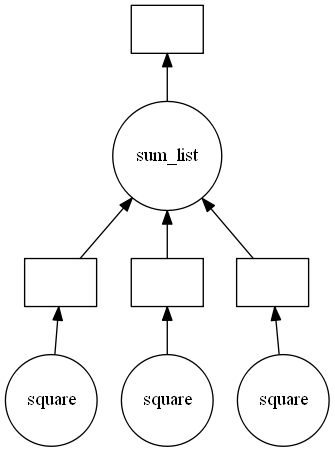
\includegraphics[width=.3\textwidth]{pic/daskgrahpdemo}
\end{center}

\begin{lstlisting}[style=incellstyle]
print("Result", computation_graph.compute())
\end{lstlisting}


\begin{lstlisting}[style=outcellstyle]
square fn:square fn:square fn: 3

 1

 2

sum_list fn: [1, 4, 9]
Result 14

\end{lstlisting} 